\documentclass[conference]{IEEEtran}
\IEEEoverridecommandlockouts
% The preceding line is only needed to identify funding in the first footnote. If that is unneeded, please comment it out.
\usepackage{cite}
\usepackage{amsmath,amssymb,amsfonts}
\usepackage{algorithmic}
\usepackage{graphicx}
\usepackage{textcomp}
\usepackage{xcolor}

\def\BibTeX{{\rm B\kern-.05em{\sc i\kern-.025em b}\kern-.08em
    T\kern-.1667em\lower.7ex\hbox{E}\kern-.125emX}}
\begin{document}

\title{Multi-Agent Reinforcement Learning Benchmark on Highway Environment for Autonomous Driving\\}


\author{\IEEEauthorblockN{Charbel Abi Hana}
\IEEEauthorblockA{\textit{M1 International Track in Electrical Engineering} \\
\textit{Université Paris-Saclay}\\
Paris, France \\
charbel-a-h@outlook.com}
}

\maketitle

\begin{abstract}
The rise of deep learning paved the way for the development of deep Reinforcement Learning methods in control, navigation and autonomous driving.
The domain of Reinforcement Learning (RL) has become a powerful learning framwork capable of learning complex policies in high-dimensional environments. In this research project
we aim to benchmark some of the widely used deep reinforcement learning methods on a simulated multi-agent highway environment. We will benchmark two decentralized algorithms; \textbf{IDQN} and \textbf{IPPO} 
which will control autonmously driven vehicles in a high density and high speed highway full of road (human driven) vehicles.  
\end{abstract}

\begin{IEEEkeywords}
Reinforcement Learning, Autonomous Driving, IDQN, IPPO
\end{IEEEkeywords}

\section{Introduction}
Autonomous driving systems constitute of multiple perception level tasks that have now achieved high precision on account of deep learning architectures. 
Besides the perception, autonomous driving systems constitute of multiple tasks where classical supervised 
learning methods are no more applicable. First, when the prediction of the agent's action changes future 
sensor observations received from the environment under which the autonomous driving agent operates, for 
example the task of optimal driving speed in an urban area. Second, supervisory signals such as time 
to collision, lateral error with respect to optimal trajectory of the agent, represent the dynamics of the 
agent, as well uncertainty in the environment. Such problems would require defining the stochastic cost 
function to be maximized. Third, the agent is required to learn new configurations of the environment, as 
well as to predict an optimal decision at each instant while driving in its environment. 
This represents a high dimensional space given the number of unique configurations under which the agent and environment are observed, this is combinatorially
large. In such cases, we will solve the decision making process by formalizing it under the classical settings of Reinforcement Learning where an agent is required
to optimally act in a given environment given a representation of that environment at a certain time step. The optimal set of actions taken by the agent is called the policy.
In this research project, we will define the basic building blocks of a Reinforcement Learning algorithm, provide two implementations of those algorithms which leverage deep learning
through multi-layered perceptron or convolution neural networks like the \textbf{IDQN} and \textbf{IPPO} which are direct extensions of the well-known Deep-Q-Learning (DQN\cite{https://doi.org/10.48550/arxiv.1312.5602}) and Proximal Policy Optimization (PPO\cite{https://doi.org/10.48550/arxiv.1707.06347}) respectively on a multi-agent level.
The performance of each algorithm will be tested on an OpenAI Gym environment called \textit{Highway-env} which simulates real world driving on an n-lane highway.

\section{Background}

\subsection{Reinforcement Learning}
Reinforcement Learning is a Machine Learning discipline where it uses many well-established methods of supervised learning such as deep neural networks for function approximation, stochastic gradient descent and backpropagation to learn data representations.

\begin{figure}[htbp]
\centerline{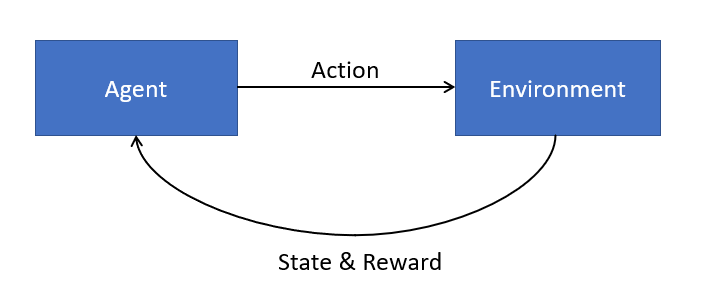
\includegraphics[width=60mm]{images/rl_diag.png}}
\caption{Generic Reinforcement Learning algorithm diagram}
\label{fig5}
\end{figure}
Reinforcement learning models learn from an environment. The environment has a set of rules and is usually assumed to be deterministic. A reinforcement learning model interacts with the environment through an agent. The agent has a state in the environment, and the agent can perform actions that change the state of the agent in the environment.
When the agent takes an action, the environment will receive this as an input and will output the resulting state and a reward (see diagram above). In other machine learning problems we usually start by defining a loss function, then we look to optimize. In reinforcement learning, we cannot immediately do that. To help us formulate a loss, we can start by looking at the rewards given back by the environment.
An agent interacts with an environment through actions, these actions change the state of the environment. The goal of the model is to determine what actions will lead to the maximum reward.

To determine the best action, reinforcement learning works by estimating the value of actions. The value of an action indicates how good an action is.
The value of an action is defined as the sum of the immediate reward received by taking an action plus the expected value of the resulting state multiplied by a scaling term. In other words, the value of an action is how good the next state will be after taking that action, plus the expected future reward from that new state.
Reinforcement learning models update their value function by interacting with the environment, choosing an action, looking at the new state, looking at the reward then updating.

Aside from the value function, the model needs to learn a policy.
The policy of the algorithm is how it chooses what action to take based on the value of the current state.
Reinforcement learning algorithms want to evaluate states as best as possible (value function) to help them make decisions (policy) that lead to the maximum reward.
\subsection{Multi-Agent Reinforcement Learning}
Multi-agent reinforcement learning studies how multiple agents interact in a common environment. That is, when these agents interact with the environment and one another, can we observe them collaborate, coordinate, compete, or collectively learn to accomplish a particular task. It can be further broken down into three broad categories:
\begin{itemize}
    \item Cooperative: All agents working towards a common goal
    \item Competitive: Agents competing with one another to accomplish a goal
\end{itemize}

Some mix of the two In addition, we can represent multi-agent problems in a centralized algorithm that communicates with the agents in the environment making all of their respective observations constantly available to the central algorithm. Another aproach, which has shown more promise, is to consider each agent as an independent agent and each agent learns based on the reward function which deviates the training to a shared objective.
\subsection{Q-Learning/Deep Q-Learning}
Reinforcement learning is all about the value function (how good our state/actions are). The models learn sequentially by integrating with the environment for a number of episodes. Episodes can be thought of as epochs in reinforcement learning, and in the chess example they would indicate the number of complete games the agent trains for.
\subsubsection{Tabular Q-Learning}
Q-learning is an off policy reinforcement learning algorithm that seeks to find the best action to take given the current state. It's considered off-policy because the q-learning function learns from actions that are outside the current policy, like taking random actions, and therefore a policy isn't needed. More specifically, q-learning seeks to learn a policy that maximizes the total reward.

The $q$ in q-learning stands for quality. Quality in this case represents how useful a given action is in gaining some future reward.

When q-learning is performed we create what's called a q-table or matrix that follows the shape of [state, action] and we initialize our values to zero. We then update and store our q-values after an episode. This q-table becomes a reference table for our agent to select the best action based on the q-value. An agent interacts with the environment in 1 of 2 ways. The first is to use the q-table as a reference and view all possible actions for a given state. 
The agent then selects the action based on the max value of those actions. This is known as exploiting since we use the information we have available to us to make a decision.

The second way to take action is to act randomly. This is called exploring. Instead of selecting actions based on the max future reward we select an action at random. Acting randomly is important because it allows the agent to explore and discover new states that otherwise may not be selected during the exploitation process. We can balance the exploration/exploitation by adjusting the discount factor shown in the formula below:

\begin{equation}
    {Q}^{new}(s_{t}, a_{t}) \leftarrow {Q}^{old}(s_{t}, a_{t}) + \alpha * (r_{t} + \lambda*\max Q(s_{t+1}, a) - Q(s_{t}, a_{t}))
\end{equation}

Where, 
\begin{itemize}
    \item ${Q}^{old}(s_{t}, a_{t})$ is the old value
    \item $\alpha$ is the learning rate
    \item $r_{t}$ is the current reward
    \item $\lambda$ is the discount factor
    \item $\max Q(s_{t+1}, a)$ is the estimate of optimal future value
\end{itemize}

\subsubsection{Deep Q-Learning}
The Q-learning method that we've reviewed above solves the issue with iteration over the full set of states in the environment, but still can struggle with situations when the count of the observable set of states is very large. As a solution to this problem, we can use a nonlinear representation that maps both state and action onto a value. In machine learning this is called a \textbf{regression problem}. The concrete way to represent and train such a representation can vary, 
but, we will be using a deep neural network with Conolutional layers and Dense layers. We will be building on top of a DQN implementation developed by PFRL library\cite{JMLR:v22:20-376}.
The algorithm for the Deep Q-learning method is shown below.

\begin{figure}[htbp]
\centerline{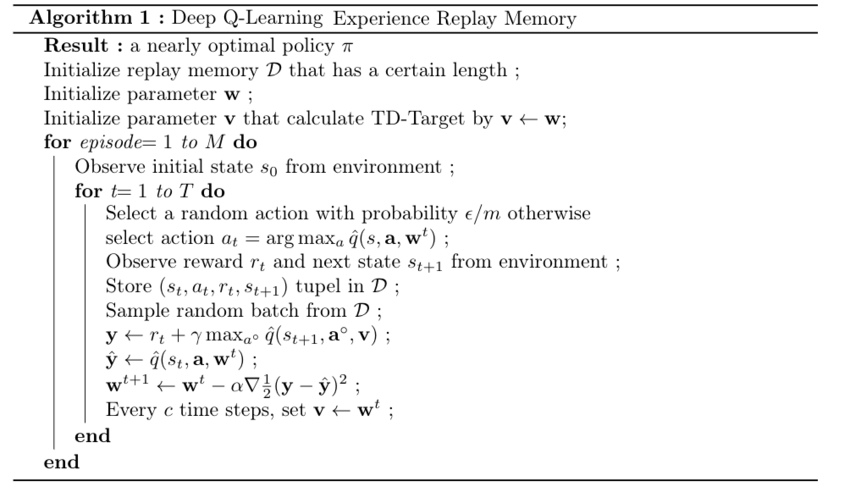
\includegraphics[width=1.0\linewidth]{images/DQN-Algorithm.png}}
\caption{Deep Q-Learning Algorithm}
\label{fig4}
\end{figure}

\subsection{Proximal Policy Optimization}
Policy gradient methods work by computing an estimator of the policy gradient and plugging it
into a stochastic gradient ascent algorithm. The optimization objective of Policy Gradient methods defined as following:

\begin{equation}
    {L}^{PG}(\theta) = {\hat{\mathbb{E}}}_{t}[\log\pi_{\theta}({a}_{t} | {s}_{t})\hat{A}_{t}]
\end{equation}

Where,
\begin{itemize}
    \item ${L}^{PG}(\theta)$ is the policy loss
    \item $\log\pi_{\theta}({a}_{t} | {s}_{t})$ is the $\log$ of the probabilities from the output of the policy network
    \item $\hat{A}_{t}$ is the estimate of the relative value of selected action.
\end{itemize}

The policy $\pi_{\theta}$ is the neural network that takes the state observation from an environment as input and suggests actions to take as an output.
The advantage is an estimation, hence the hat over A, of the relative value for selected action in the current state. It is computed as a discounted reward (Q) — value function, where the value function basically gives an estimate of discounted sum of reward. When training, this neural net representing the value function will frequently be updated using the experience our agent collects in an environment.
As much appealing it is to constantly perform gradient descent steps in one batch of collected experience, it will often update the parameters so far outside of the range that leads to \textbf{destructively large policy updates}.
\subsubsection{Trust Region Policy Optimization}
One of the approaches to prevent such destructive policy updates was Trust Region Policy Optimization\cite{https://doi.org/10.48550/arxiv.1502.05477}.
In this paper, the authors implemented an algorithm to limit the policy gradient step so it does not move too much away from the original policy, causing overly large updates that often ruin the policy altogether.
\subsubsection{Clipped Surrogate Objective}
Proximal Policy Optimization attempts to simplify the optimization process while retaining the advantages of TRPO.
One of this paper's main contribution is the clipped surrogate objective:
\begin{equation}
    {L}^{PG}(CLIP) = {\hat{\mathbb{E}}}_{t}[\min({r}_{t}(\theta)\hat{A}_{t},clip({r}_{t}(\theta), 1-\epsilon, 1+\epsilon)\hat{A}_{t})]
\end{equation}
Here, the expectation over a minimum of two terms is computed: normal PG objective and clipped PG objective. The key component comes from the second term where a normal PG objective is truncated with a clipping operation between 1-epsilon and 1+epsilon, epsilon being the hyperparameter.
The final loss function by summing this clipped PPO objective and two additional terms:
\begin{equation}
    {L}^{PG}(CLIP+VF+S) = {\hat{\mathbb{E}}}_{t}[L^{CLIP}_{t}(\theta) - c_{1}L^{VF}_{t}(\theta) + c_{2}S[\pi_{\theta}](s_{t})]
\end{equation}
The $c_{1}$ and $c_{2}$ are hyperparameters. The first term is a mean square error of the value function in charge of updating the baseline network. The second term, which may look unfamiliar, is an entropy term used to ensure enough exploration for our agents. This term will push the policy to behave more spontaneously until the other part of the objective starts dominating.
The algorithm altogether for multiple epoch updating is shown below in figure 3.

\begin{figure}[htbp]
\centerline{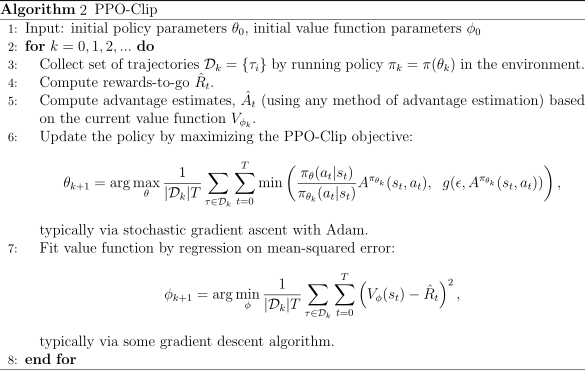
\includegraphics[width=1.0\linewidth]{images/ppo_algorithm.png}}
\caption{Proximal Policy Optimization Algorithm}
\label{fig6}
\end{figure}

\section{Environment}
The environment used in this research project is \textit{highway-env}\cite{highway-env}. This environment is a minimalist python implementation of a highway simulation. There is a multitude of environments present in the package provided by the developers.
Their environments are based on OpenAI Gym\cite{brockman2016openai}.

\begin{figure}[hbt!]
\vspace*{0.1cm}
\centerline{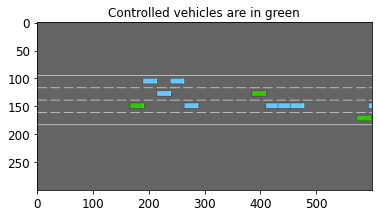
\includegraphics[width=75mm]{images/highway-env.png}}
\caption{Highway Environment in multi-agent configuration}\label{fig1}
\end{figure}

\subsection{Action Space}
The actions shown in figure 5 below represent the discrete action space of any RL agent. The availability of these actions depends on the positioning of the agent in the environment
(lane changes at the edges of the roads, or accelerating/decelerating beyond the maximum velocity). Taking an unavailable action is equivalent to taking the \textit{IDLE} action.
Taking an unavailable action is equivalent to taking the \textit{IDLE} action.
\begin{figure}[hbt!]
\centerline{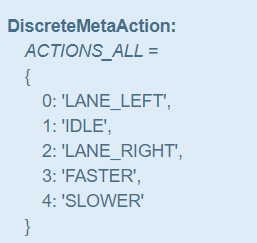
\includegraphics[width=0.3\linewidth]{images/action_space.png}}
\caption{Generated Output after 100 Steps}
\label{fig2}
\end{figure}

\subsection{Observation Space}
We'll be using the \textit{KinematicObservation} which essentially is  $V*F$  array where  $V$ represents a list of nearby vehicles and  $F$  represents the feature being the  $x-y$  positions, velocities and orientation of the autonomously-driven
vehicles and the road (human-driven) vehicles. One feature vector has the following elements:
\begin{itemize}
    \item $presence$: 0/1, Disambiguate agents at 0 offset from non-existent agents.
    \item $x$: World offset of ego vehicle on the x axis.
    \item $y$: World offset of ego vehicle on the y axis.
    \item $v_{x}$: Velocity on the x axis of vehicle.
    \item $v_{y}$: Velocity on the y axis of vehicle.
    \item $\cos_{h}$: Trigonometric heading of vehicle.
\end{itemize}
A sample of the observation (limited to velocity and positioning) is shown in figure 6 below.
\begin{figure}[hbt!]
\centerline{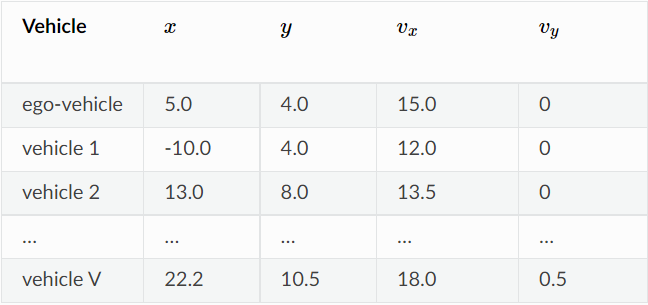
\includegraphics[width=80mm]{images/observation_space.png}}
\caption{KinematicObservation observation space sample}
\label{fig3}
\end{figure}

\subsection{Reward}
The general focus is on two features: a vehicle should progress quickly on the road and should avoid collisions. Thus, the reward function is often composed of a velocity term and a collision term:\\ 
\begin{equation}
    R(s,a) = a * \frac{v - {v}_{\min}}{{v}_{\max}-{v}_{\min}} - b * {collision}
\end{equation}
where  $v$, ${v}_{\min}$ and ${v}_{\max}$  are the current, minimum and maximum speed of the ego-vehicle respectively, and  $a$, $b$  are two configurable coefficients.
It should be noted that we can wrap this reward function through Gym's \textit{RewardWrapper} inheritence class and we can change the definition of the reward. However, we will refrain for this research project
as the objective is to benchmark decentralized algorithms on this environment.

\section{Experimentation and Results}

\subsection{Environment Configuration}
The main configurable parameters of the environment here are:
\begin{itemize}
    \item $controlledVehicles$: number of RL agents; 3
    \item $ObservationType$: Kinematic
    \item $features$: $[presence, x, y, v_x, v_y, \cos_h]$
    \item $vehiclesCount$: number of human-driven vehicles; 10
    \item $vehicleDensity$: density of human-driven vehicles; 5
\end{itemize}

The main training loop for any implemented algorithm on our configured environment is shown in figure 7.

\begin{figure}[hbt!]
\centerline{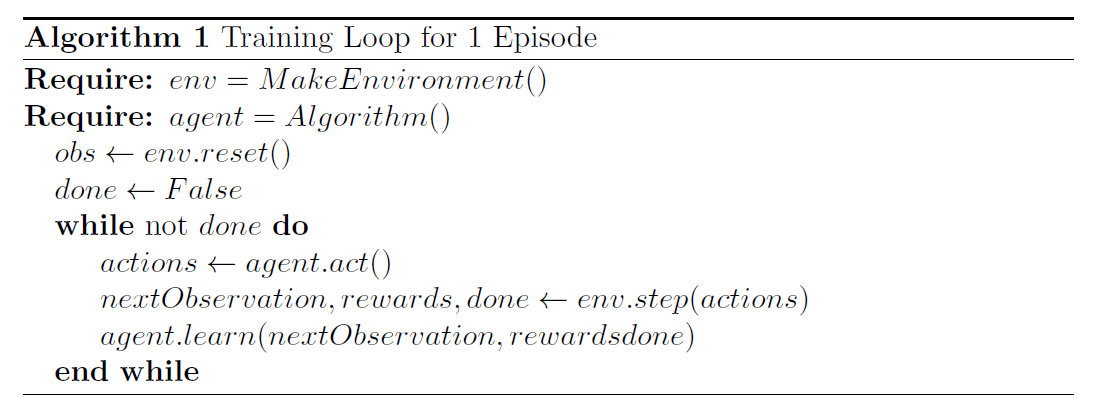
\includegraphics[width=1.0\linewidth]{images/gym_loop.png}}
\caption{General Gym Environment training loop}
\label{fig10}
\end{figure}

\subsection{Evaluation Metrics}
In this research project, we will mainly use the \textit{avg\_reward} on all 3 agents and we will aggregate a \textit{score} metric
which keeps track of the summed rewards over one episode. 

\subsection{Decentralized Algorithms}
As mentioned previously, the two algorithms used for this benchmark are direct extensions of the DQN and IPPO models. We develop the IDQN and IPPO
models by initializing for each agent in the environment its own network. The observations perceived by each agent may contain information about other agents
however, communication and rewards sharing isn't implemented. The agents are fully independent in this case.\\
For the IDQN model, we use the following network;
\begin{itemize}
    \item Observation matrix enters a 2D Convolution layer with 64 feature maps and kernel size $(2, 2)$
    \item Output is followed by LeakyReLU activation function and a flattening layer
    \item A multi-layer perceptron block is followed with units of 64 and 5 (action space size) with ReLU activation in the hidden layer and a DisceteActionValueHead layer from PFRL for outputing probabilities mapped to the action space.
\end{itemize}

For the IPPO model, we use the same backbone network with a change to the output head being a SoftmaxCategoricalHead which is also provided by PFRL.
All the other hyperparameters are left to their default values.
\subsection{Results}
After training both models on the same environment configurations we obtain the following results (figures 8 and 9) of the score per episode for the IDQN model (on the right) and the IPPO model (on the left).
The IDQN models showed higher score values comapred to the IPPO models with scores reaching 17 and 5 respectively. When both models are trained for 1000 episodes
we can clearly see the noise in the obtained result as both algorithms are extremly sensitive to hyperparameter and some tuning can be done to obtain a better augmenting trend in both scores.
\begin{figure}[hbt!]
    \vspace*{0.2cm}
    \centering
    \begin{minipage}[b]{1.0\linewidth}
      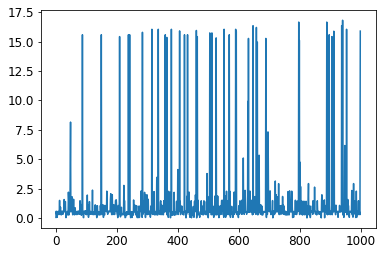
\includegraphics[width=\textwidth]{images/idqn-res.png}
      \caption{Score in function of episodes for IDQN model}
    \end{minipage}
    \hfill
    \begin{minipage}[b]{1.0\linewidth}
      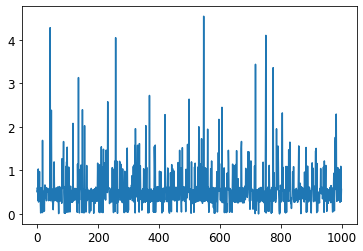
\includegraphics[width=\textwidth]{images/ppo_res.png}
      \caption{Scores in function of episodes for IPPO model}
    \end{minipage}
  \end{figure}

\section{Conclusion}
In this research project, we attempted to deploy autonomously driven cars in a dense highway environment using deep reinforcement learning methods. The development in this field also contributes to other
issues like decreasing CO2 emmissions through efficient road navigation, reducing overall traffic congestions and organising intersections. With the current rise in the trend of autonomous vehicles
benchmarks similar to the one we present are used as a pointer of performance in different environments and different conditions as we continousky aim to generalize machine learning and deep learning models
on new and unseen environments and data. The field of deep Reinforcement Learning is showing extreme promise in the industry due to the extreme devotion to research. Future additions to this work 
can include centralized algorithms on the same environment where an orchestrator with visibility on all agents data controls their actions simultaneously.

\bibliographystyle{ieeetr} % We choose the "plain" reference style
\bibliography{citations} % Entries are in the refs.bib file
\end{document}
